
\section*{\textbf{\underline{Abstract}}}
The dispersal of individuals between spatially distributed populations is key for the maintenance of metapopulations and local populations. In this case, differences in the level of isolation of patches within spatial networks can have contrasting effects on their resulting dynamics, influencing the size, variability, and persistence time of metapopulations. We experimentally examined how the degree distribution of spatial networks influences the size, variability, and persistence of \textit{Daphnia} metapopulations. We found that spatial networks that are more heterogeneous have longer persistence times than homogeneous networks, but their size and variability is the same across different network types. At the local population level, patch degree did not influence the size, variability, and probability of a patch being occupied. These results suggest that degree distribution has complex effects on metapopulation dynamics.

%-----------------------
\section*{\textbf{\underline{Introduction}}}

The dispersal of individuals between spatially distributed populations has important effects on populations \parencite{hanski1998, abbott2011}, influencing colonization-extinction dynamics, the variability of local populations, and metapopulation persistence \parencite{wang2015,fox2017, schmidt2020}. The spatial distribution and distance between populations affect the probability of individual dispersal in spatial networks, such that individuals are less likely to disperse to more isolated populations, which can increase the extinction risk of these populations \parencite{brown1977, schmidt2020}. Population sizes also also play a key role in driving local dynamics, where smaller populations are more likely to vary and go extinct, even in homogeneous environments, because of demographic stochasticity \parencite{hanski1998,melbourne2008}. Dispersal of individuals may thus be crucial for the maintenance of small populations \parencite{sutherland2012}.
%to allow the persistence of species that have small population sizes
 
%The spatial distribution of populations across landscapes is an important determinant of local population dynamics through dispersal events \parencite{hanski1998}. Dispersal of individuals influence colonization-extinction dynamics, the variability of local populations, and metapopulation persistence \parencite{fox2017}. The spatial distance between populations affect the dispersal of individuals in these spatial networks, such that fewer individuals would disperse to more isolated populations leading to a higher extinction rates in these areas \parencite{macarthur1970, brown1977, schmidt2020}. Local population sizes would also influence these dynamics, such that smaller populations would be more likely to vary and go extinct, even in homogeneous environments, because of demographic stochasticity \parencite{hanski1998,melbourne2008}. This suggests that dispersal is particularly important to allow the persistence of species that have small population sizes \parencite{sutherland2012}.
\paragraph*{}
%Although small populations face higher extinction risk, the persistence of these populations in spatial networks can be enhanced through dispersal events that provide a continuous influx of individuals and prevent their local extinction, through the rescue effect, and enhance metapopulation persistence \parencite{brown1977, abbott2011}. Talk about panmitic patchy metapops here and how dispersal may vary in these cases? Classical metapopulation theory states that individuals can only disperse to some of the populations, but empirical evidence rarely support this, and instead, it seems that patchy panmitic metapopulations are common
Rare and common species, when occurring in ecologically marginal environments, have populations with low densities \parencite{brown1984, lawton1993}, such that small populations are prevalent in nature and represent a key component of biodiversity \parencite{preston1948,ehrlich1993}. Although small populations face higher extinction risk, dispersal can provide a continuous influx of individuals to small populations and prevent their local extinction in spatial networks, through the rescue effect, and enhance metapopulation persistence \parencite{brown1977, abbott2011}. The prevalence of dispersal events in spatial networks can widely vary to being relatively rare in classic metapopulations to being extremely common in patchy populations \parencite{elmhagen2001, ovaskainen2004, fronhofer2012}. Theoretical frameworks indicate that such differences in dispersal across networks can lead to substantially different dynamics in metapopulations and local populations \parencite{heino1997,abbott2011,gilarranz2012,wang2015}, though there is mixed evidence from empirical systems supporting these theoretical predictions \parencite{yang2022}. 

% In patchy populations dispersal events are frequent such that the same individual may reproduce in different patches during its life time \parencite{harrison1991, ovaskainen2004}. Patchy populations represent an interesting framework to understand the effects of isolation on population dynamics given that patches can vary in their degree of accessibility, but still be reachable by all individuals.% This would allow 
%Why are patchy populations interesting? 
% depending on the spatial structure of the local populations \parencite{} According to classic metapopulation theory, the dispersal of individuals between populations is a relatively rare event    However, high dispersal rates may promote synchrony between populations and might negatively impact metapopulation persistence by increasing the probability that local populations go extinct simultaneously \parencite{heino1997,abbott2011}. Although dispersal is predicted to decrease local population variability \parencite{abbott2011,wang2015}, experimental evidence supporting this expectation is contrasting, indicating that the effects of dispersal on local population variability may vary across taxa and depend on experimental length \parencite{yang2022}.  
%Experimental evidence show that taxa, number of patches, and experimental length influence the observed effects of dispersal on population dynamics \parencite{yang2022}, further highlighting that dispersal can have complex effects on population dynamics.  

\paragraph*{}
The spatial distance between populations across landscapes is often used to represent population isolation, but the degree distribution (i.e., number of connections that populations share in a network) also provides information on their level of isolation \parencite{schmidt2020,arancibia2021}. Populations occurring in real networks have different number of connections that directly influence their dynamics \parencite{hanski1998, arancibia2024}. For instance, metapopulations that have sites that are heterogeneous in their number of connections may be able to persist under a winder range of scenarios than homogeneous metapopulations \parencite{artzy2010, grilli2015}, though species life-history traits may affect how these dynamics unfold \parencite{gilarranz2012}. Local population dynamics can also be influenced by patch degree, where patches may be less variable and more often occupied when they are highly connected \parencite{gilarranz2012, arancibia2024}. This suggests that differences in network topology caused by how the number of connections are distributed across nodes, and consequently by how isolated patches are, can substantially affect metapopulation and local population dynamics even when everything else, such as resource availability and environmental conditions, remains constant.

%in metacommunities, a positive relationship between number of connections and community variability is observed when communities have a high variation in the number of connections, but not when the number of connections is similar across communities \parencite{arancibia2024}. 


\paragraph*{}
Here we experimentally examined how the degree distribution of spatial networks influences the size, variability, and persistence of \textit{Daphnia} metapopulations. These spatial networks were composed of  small extinction-prone populations that were identical, but could have one of three types of degree distribution (Figure \ref{fig:conceptual}). We hypothesized that metapopulations that were more heterogeneous in their degree distribution would be larger, less variable, and persist for longer periods of time than more homogeneous metapopulations. We also predicted that local populations would be larger, less variable, and more likely to be temporally occupied the more connections populations had. We found that spatial networks that are more heterogeneous have longer persistence times than homogeneous networks, but their size and variability is the same across different network types. At the local population level, patch degree did not influence the size, variability, and probability of a patch being occupied. 
% local variability would be lowest in populations that have an intermediate number of connections while metapopulation persistence would be enhanced in spatial networks where populations are variable in their number of connections. This was expected because intermediate dispersal is often suggested to reduce population variability \parencite{abbott2011} and because a high variation in number of connections may prevent synchrony between populations and enhance metapopulation persistence \parencite{arancibia2024}. We found.. 

%%%The environmental correlation of the patches may influence the effects of dispersal on population variabilioty


%estimate CV using all information and estimate it considering only cases when patches were occupied to see if results change. When using all data we may need to take the log?
%Degree distribution affected the variability of metacommunities when communities had a high variation in the number of connections, but not when communities had a similar number of connections \parencite{arancibia2024}.    where populations have on average the same number of connections the number of connectes  BREAK DOWN THIS PART

% Alternatively, increasing the mean number of connections between populations in a network may enhance metapopulation persistence \parencite{holyoak2000}, but can also promote synchrony between populations and increase metapopulation extinction risk \parencite{}. This indicates that number of connections can have a complex effect on metapopulation dynamics. 

%spatial networks that higher higher mean number of connections may have positive effects on metapopulation persistence promote synchrony between populations and increase metapopulation extinction risk \cite{refs}. 

%For instance, spatial networks where patches are equally connected may promote synchrony between populations and increase metapopulation extinction risk \cite{refs}. 

%  natural world isolation of populations in spatial networks are often 
%Although geographic distance between populations is often used to estimate the isolation of populations \parencite{schmidt2020}, populations may be more or less isolated depending on how many others are connected to them. Talk about degree distribution here


%Talk about network structure and degree in here. It has been not investigated that much in experiments and blablabla
%Early on theoretical models of patch networks considered all patches being equally connected, but this is not the case in real networks \parencite{hanski1998} 
% Isolation may not necessarily be measured by distance, but by the degree
 
%Local population dynamics are influenced by the spatial distribution of populations across geographic space, such that complex spatial dynamics can be observed even in the absence of environmental heterogeneity \parencite{hanski1998}. For instance, demographic stochasticity can be an important driver of population dynamics when population sizes are small, and that may to lead to complex extinction and recolonization dynamics occur  \parencite{melbourne2008,la,lw}. 

%end paragraph wioth dispersal

%Complex spatial dynamics in populations can be observed even in the absence \paragraph*{}
%This paragraph is about the effects of dispersal on meta population stability and persistence

%-----------------------
\section*{\textbf{\underline{Methods}}}

\paragraph*{Experimental system}\mbox{}\\
Our model species consists of a single clone of the freshwater cladoceran \textit{Dahpnia dentifera} reared on a mixture of filtered lake water and deionized water. To remove the potential confounding effects that individual age and maternal environment could have on vital rates, we isolated offspring from parthenogenetic females raised in isolation to obtain individuals of known age and maternal environment. Parthenogenetic females were individually placed into 50 mL test tubes filled with filtered lake water and deionized water, and were daily fed 50 $\mu$g  of a 2 g/L suspension (equivalent to 1 mg/L algal dry weight) of pulverized blue-green algae (\textit{Spirulina sp.}) and kept on the laboratory benchtop under a 12 hour light cycle. A total of 720 individuals that were 2-3 days old were obtained to seed the spatial networks (see details below).

%\textit{D. dentifera} were fed 50 $\mu$g  of a 2 g/L suspension (equivalent to 1 mg/L algal dry weight) of pulverized blue-green algae (\textit{Spirulina sp.}), and kept on the laboratory benchtop under a 12 hour light cycle.

%To remove the potential confounding effects that individual age and maternal environment could have on vital rates, we isolated offspring from parthenogenetic females raised in isolation to obtain individuals of known age and maternal environment. Parthenogenetic females were individually placed into 50 mL test tubes filled with filtered lake water and deionized water and were daily fed 50 $\mu$g  of a 2 g/L suspension (equivalent to 1 mg/L algal dry weight) of pulverized blue-green algae (\textit{Spirulina sp.}). We obtained 720 individuals that were 1-3 days old that where used in the 30 metapopulations that we considered in our study. 
\paragraph*{Spatial networks}\mbox{}\\
To examine how degree distribution influence local population dynamics and the persistence of \textit{D. dentifera}, we created three spatial network types (ten replicates per type; Figure 1) composed of 24 patches of size $\approx$ 2.5mL that had the same edge density (number of dispersal corridors, 36), but that the degree distribution (number of corridors per patch) changed across the spatial network types. In the first network type, the degree distribution was homogeneous across patches, and every patch was connected to three other patches (hereafter low networks, Figure \ref{fig:conceptual}a). In the second network type, there was some heterogeneity in the degree distribution, such that most patches were connected to to two or five other patches (hereafter mid networks, Figure \ref{fig:conceptual}b). In the third network type, the degree distribution was highly heterogeneous where patches widely varied in their degree, ranging from one to eight connections (hereafter high networks, Figure \ref{fig:conceptual}c).
 
The experiment started with all patches in the spatial networks being occupied by one individual, such that each network had 24 individuals at the beginning of the experiment. Spatial networks were fed pulverized blue green algae daily and kept under a 12 hour light cycle. The number of individuals in each patch was counted daily for 104 days, and a network was considered extinct when no individuals were detected in any patch for three consecutive days. We considered day 104 to be the extinction time of metapopulations that still had individuals up to that day. 
 
\paragraph*{Estimating the size, variability, and persistence of metapopulations}\mbox{}\\
Metapopulation size was estimated as mean number of individuals recorded daily in the networks until extinctions occurred. Metapopulation variability was calculated as the coefficient of variation
(hereafter CV$_{met}$ $CV = \frac{\sigma}{\mu}$), relating the standard deviation in the density of a metapopulation ($\sigma$) to it's mean ($\mu$) density. Metapopulation variability was estimated for spatial networks considering all sampling events until extinctions were observed. Lastly, metapopulation persistence was estimated as the number of days until a spatial network went extinct. At the patch level, we estimated mean population size, population variability using the coefficient of variation (hereafter CV$_{pop}$), and we estimated temporal occupancy as the fraction of days that patches were occupied by at least one individual. 


%Local population variability was estimated using coefficient of variation (hereafter CV; $CV = \frac{\sigma}{\mu}$), relating the standard deviation in the density of a patch ($\sigma$) to it's mean ($\mu$) density. 
%[\textit{Potential problem: Can we estimate population variability with a lot of zeros as in our case? What are alternative estimates we could use?}]. We calculated metapopulation persistence time (set to a maximum values of X for the metapopulations that persisted for the whole duration of the experiment) as number of days until metapopulation extinction.

The effects of spatial network type on metapopulation size, variability, and persistence was evaluated using linear mixed effect models. In these models, the size, variability (CV$_{met}$), and persistence time (number of days) of spatial networks were used as response variable and network type was used as fixed effect while replicate number was used as random effect. Linear mixed effect models were also used to assess how the number of connections that patches had was related to their mean density, their variability in density, and to their probability of being occupied over time.  In these models, the response variable was mean population density, population variability (CV$_{pop}$), and temporal occupancy while the fixed effect was patch degree and the random effects were replicate number and patch number. These linear mixed models were fit considering a Gaussian family with the \texttt{glmmTMB} R package \parencite{brooks2017} and we estimated model goodness of fit (Nakagawa's conditional $R^2$) using the \texttt{performance} R package \parencite{ludecke2021}. This conditional $R^2$ takes fixed and random effects into account when estimating the model goodness of fit. 

% local population variability and number of connections were assessed using a linear mixed model. In this model, population variability (CV) was the response variable and degree (number of connections a patch had) was the fixed effect. We used network type and replicate as random effects. This linear mixed model was fit considering a Gaussian family with the \texttt{glmmTMB} R package \parencite{brooks2017} and we performed model diagnostics (see Figure \ref{fig:main_mod} and Supporting Information for details) and estimated model goodness of fit (Nakagawa's conditional $R^2$) using the \texttt{performance} R package \parencite{ludecke2021}. This conditional $R^2$ takes fixed and random effects into account when estimating the model goodness of fit. [\textit{Potential problem: Unbalanced number of patches with different degrees in the analyses. Specifically: Degree of 1 = 60 patches, 2 = 210 patches, 3 = 290 patches, 4 = 30 patches, 5 = 110 patches, 6 and 8  = 10 patches. What to do about this? Maybe bootstrapping? idk}]


%-----------------------
\section*{\textbf{\underline{Results}}}

\paragraph*{}
We found that metapopulation size and variability did not differ between the different network types (Figure \ref{fig:met}a-b). However, the heterogeneity in the degree distribution of networks affected their persistence time. Specifically, high networks had a longer persistence time than low, but not than mid (Figure \ref{fig:met}c), networks such that this model explained 31\% of the variance in persistence time of metapopulations (Table \ref{tab:lmm_meta}). At the patch level, degree did not influence the size, variability, and probability of patches being occupied over time (Figure \ref{fig:pop}, Table \ref{tab:lmm_pop}). 


%-----------------------



\section*{\textbf{\underline{Discussion}}}
The effects of network topology on metapopulation dynamics has long interested ecologists who have often addressed these questions using theoretical models and simulation frameworks \parencite{artzy2010,gilarranz2012,grilli2015}. However, the extent to which the findings from such theoretical studies are generalizable to empirical systems has been rarely assessed (but see \textcite{arancibia2021, arancibia2024}). Here, we experimentally examined how differences in network topology caused by variations in how connections are distributed across patches in networks affect metapopulation and local population dynamics of \textit{Daphnia dentifera}. At the metapopulation level, we found support for the expectation that increasing heterogeneity in the number of dispersal corridors that local populations have enhances metapopulation persistence. However, metapopulation size and variability were not different across network types, suggesting that metapopulation persistence may not enhanced through increases in the size and reductions in the variability of metapopulations. At the local population level, we found that patch degree did not influence mean population size, population variability, or the probability of a patch being occupied, thus not supporting our expectations. %Cite models that predicted

\paragraph*{}

The effects of degree distribution on metapopulation dynamics can depend on species life-history traits, where species that experience high extinction probabilities have superior performance in heterogeneous compared to homogeneous networks \parencite{gilarranz2012}. This might explain the increase in persistence time that we observed in our experiment as the metapopulations considered were composed of small extinction-prone populations. This could be occurring because homogeneous networks may promote density-dependent mortality as all patches are equally reachable by individuals, leading to resources being depleted more consistently and increasing the mortality in such networks. However, a relative small amount of heterogeneity in the degree distribution of networks seems to be enough to prevent this from occurring as our mid networks persisted for roughly the same amount of time as the high networks. 

\paragraph*{}
At the patch level, a high degree is often predicted increase patch temporal occupancy and to decrease population variability \parencite{gilarranz2012,arancibia2024}, though our experiment do not support these predictions. The effects of degree on local populations may be modulated by the neighbor patches. For example, patches may be more often occupied when they are linked to well connected patches than when they are linked to poorly connected patches \parencite{gilarranz2012}. This suggests that differences in patch position within networks influence local populations and could explain the high variability in the dynamics that we observed for patches that had low degree. Moreover, dispersal often has no effects on population dynamics in empirical systems \parencite{yang2022}, indicating that that degree may play a complex role in affecting local population and metapopulation dynamics. 
%shortcomings? (small metapop and perhaps they are not dispersally restricted) only a few nodes with 8 or more connections due to constraints of the networks
\paragraph*{}
We show that differences in the degree distribution of spatial networks affect different aspects of metapopulation and local population dynamics. While some of our findings confirm some theoretical predictions at the metapopulation level, differences in the degree of patches did not affect local populations. Experimentally assessing the effects of degree distribution on species that have different life-history traits than \textit{Daphnia} could improve our understanding of how differences in patch isolation affects empirical metapopulation dynamics. For example, considering species that face dispersal limitation in spatial networks could provide additional insights on how the dispersal ability of species can modulate the influence of degree distribution on metapopulation dynamics. 



\section*{\textbf{\underline{Tables}}}
% latex table generated in R 4.3.2 by xtable 1.8-4 package
% Wed Mar 12 15:31:57 2025
\begin{table}[H]
\centering
\caption[Metapopulation linear mixed effect model]{Results from linear mixed effect models that assessed how the different type of networks influenced metapopulation size, variability, and persistence.}
\begin{tabular}{cccccc}
  \hline
 Response & Degree distribution & Estimate & Std. Error & z value & pval \\ 
  \hline
  &Intercept & 98.500 & 4.342 & 22.687 & \textbf{<0.001} \\ 
  Persistence &Low & -22.200 & 6.140 & -3.616 & \textbf{<0.001} \\ 
  &Mid & -9.900 & 6.140 & -1.612 & 0.107 \\ \hline
  &Intercept & 20.028 & 1.436 & 13.945 & \textbf{<0.001} \\ 
  Size &Low & -1.161 & 2.031 & -0.572 & 0.568 \\ 
  &Mid & -1.201 & 2.031 & -0.591 & 0.554 \\ \hline
  &Intercept & 0.752 & 0.049 & 15.493 & \textbf{<0.001} \\ 
  Variability&Low & -0.029 & 0.069 & -0.424 & 0.672 \\ 
  &Mid & -0.037 & 0.069 & -0.541 & 0.588 \\ 
   \hline
\end{tabular}
\label{tab:lmm_meta}
\end{table}



% latex table generated in R 4.3.2 by xtable 1.8-4 package
% Wed Mar 12 15:38:51 2025
\begin{table}[H]
\centering
\caption[Population linear mixed effect model]{Results from linear mixed effect models on the effects of degree on patch temporal occupancy, size, and variability.} 
\begin{tabular}{cccccc}
  \hline
Response & Predictor & Estimate & Std. Error & z value & pval \\ 
  \hline
 Occupancy &Intercept & 0.418 & 0.017 & 24.920 & \textbf{<0.001} \\ 
  &Degree & -0.002 & 0.004 & -0.418 & 0.676 \\ \hline
  Size&Intercept & 0.777 & 0.047 & 16.421 & \textbf{<0.001} \\ 
  &Degree & 0.008 & 0.012 & 0.703 & 0.482 \\ \hline
  Variability&Intercept & 1.644 & 0.053 & 30.953 & \textbf{<0.001} \\ 
  &Degree & -0.010 & 0.013 & -0.753 & 0.452 \\ 
   \hline
\end{tabular}
\label{tab:lmm_pop}
\end{table}

\section*{\textbf{\underline{Figures}}}

\begin{figure}[ht]
\centering
\centerline{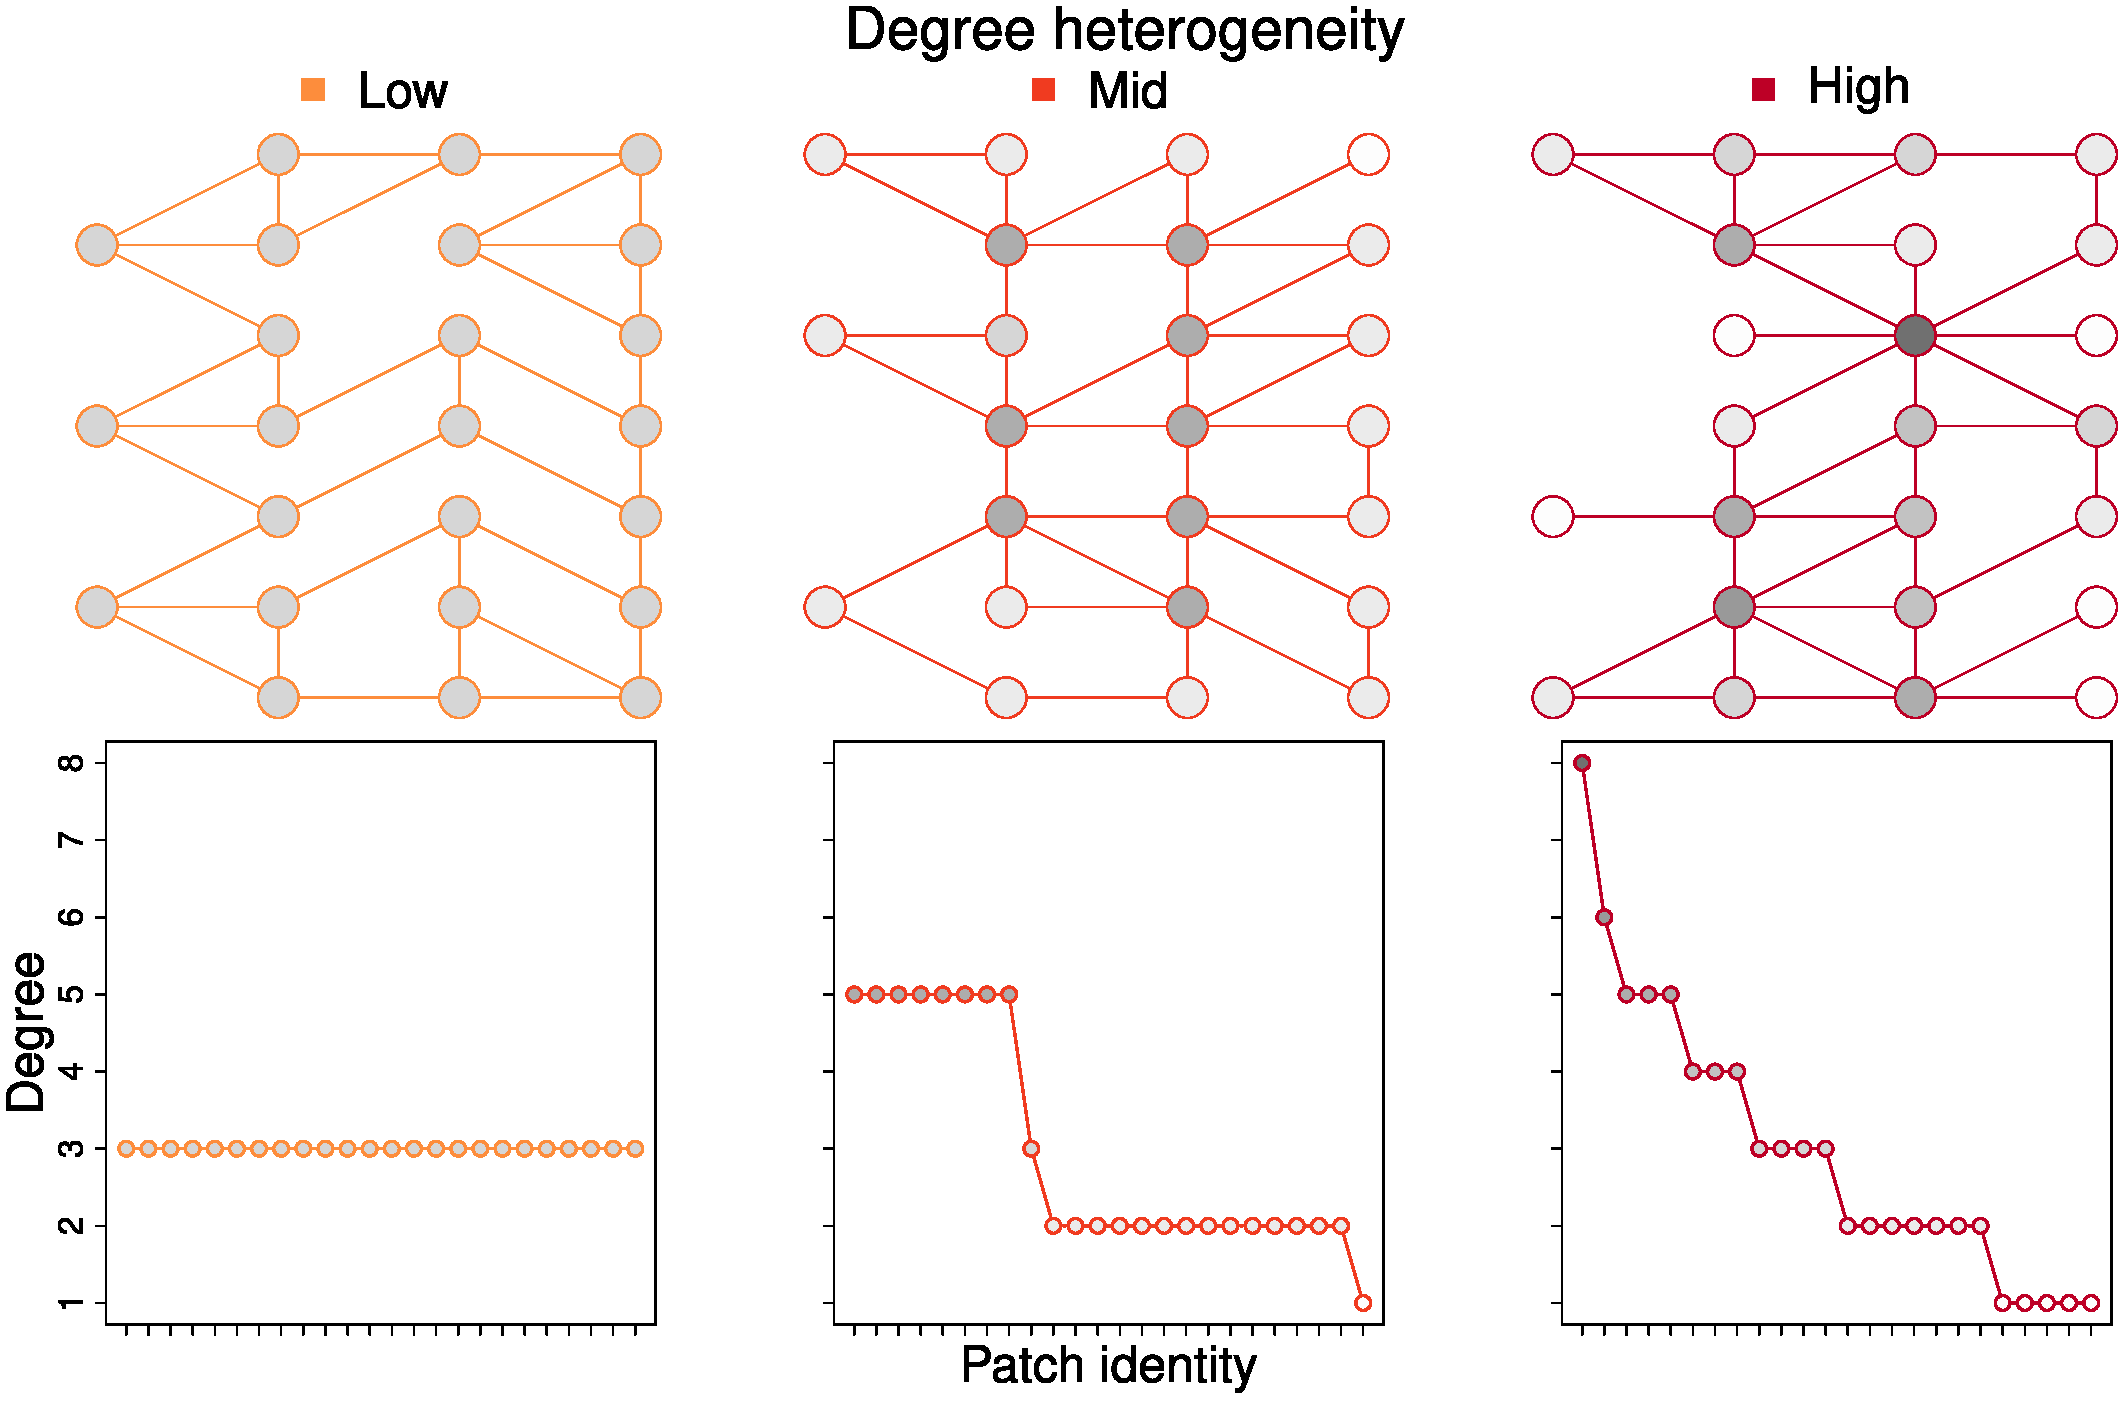
\includegraphics[width=1\textwidth]{FigSpat/concep}}
\caption[Experimental spatial networks]{Spatial networks that had different degree distribution considered in our experiment, showing a gradient of more to less homogeneous networks from left to right.} 
\label{fig:conceptual}
\end{figure}
\clearpage

\begin{figure}[ht]
\centering
\centerline{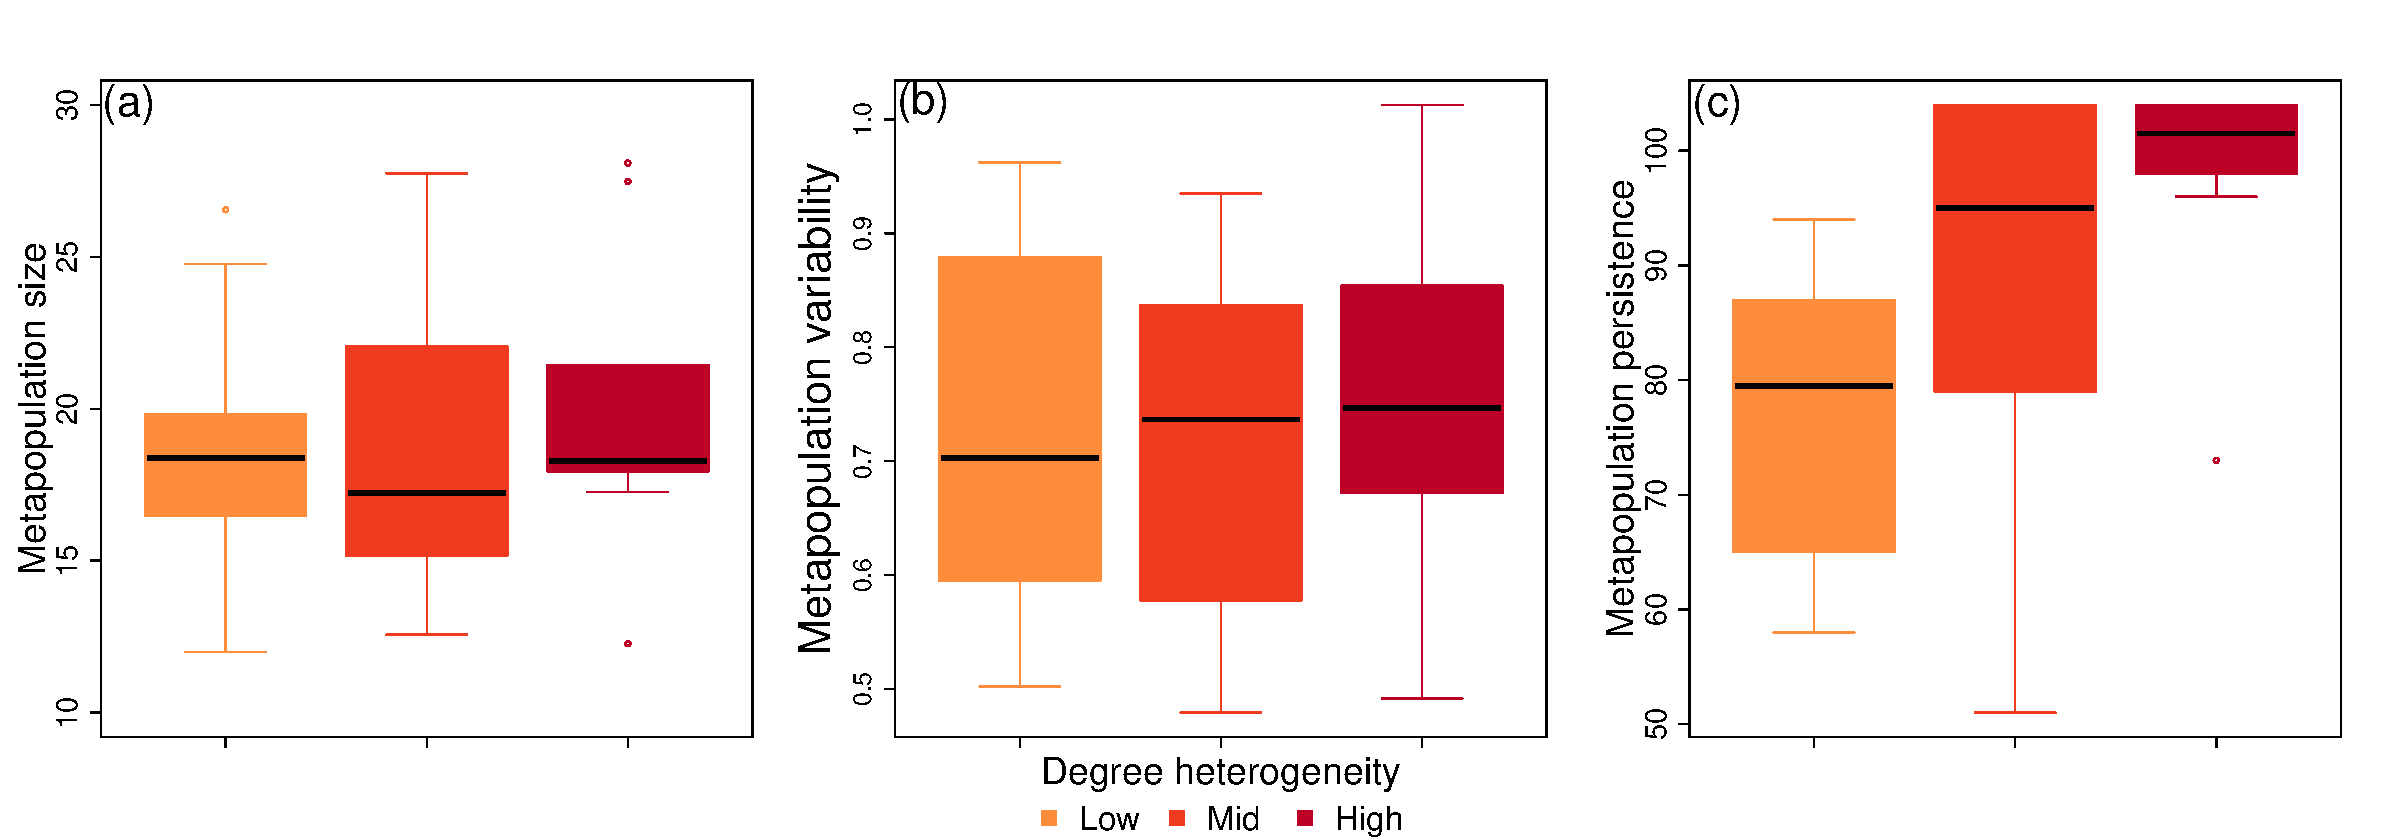
\includegraphics[width=1\textwidth]{FigSpat/meta_res}}
\caption[Effect of network type on metapopulation dynamics]{Degree distribution heterogeneity did not affect metapopulation size (a) or metapopulation variability (b), but more heterogeneous networks persisted for longer periods of time (c).} 
\label{fig:met}
\end{figure}


\begin{figure}[ht]
\centering
\centerline{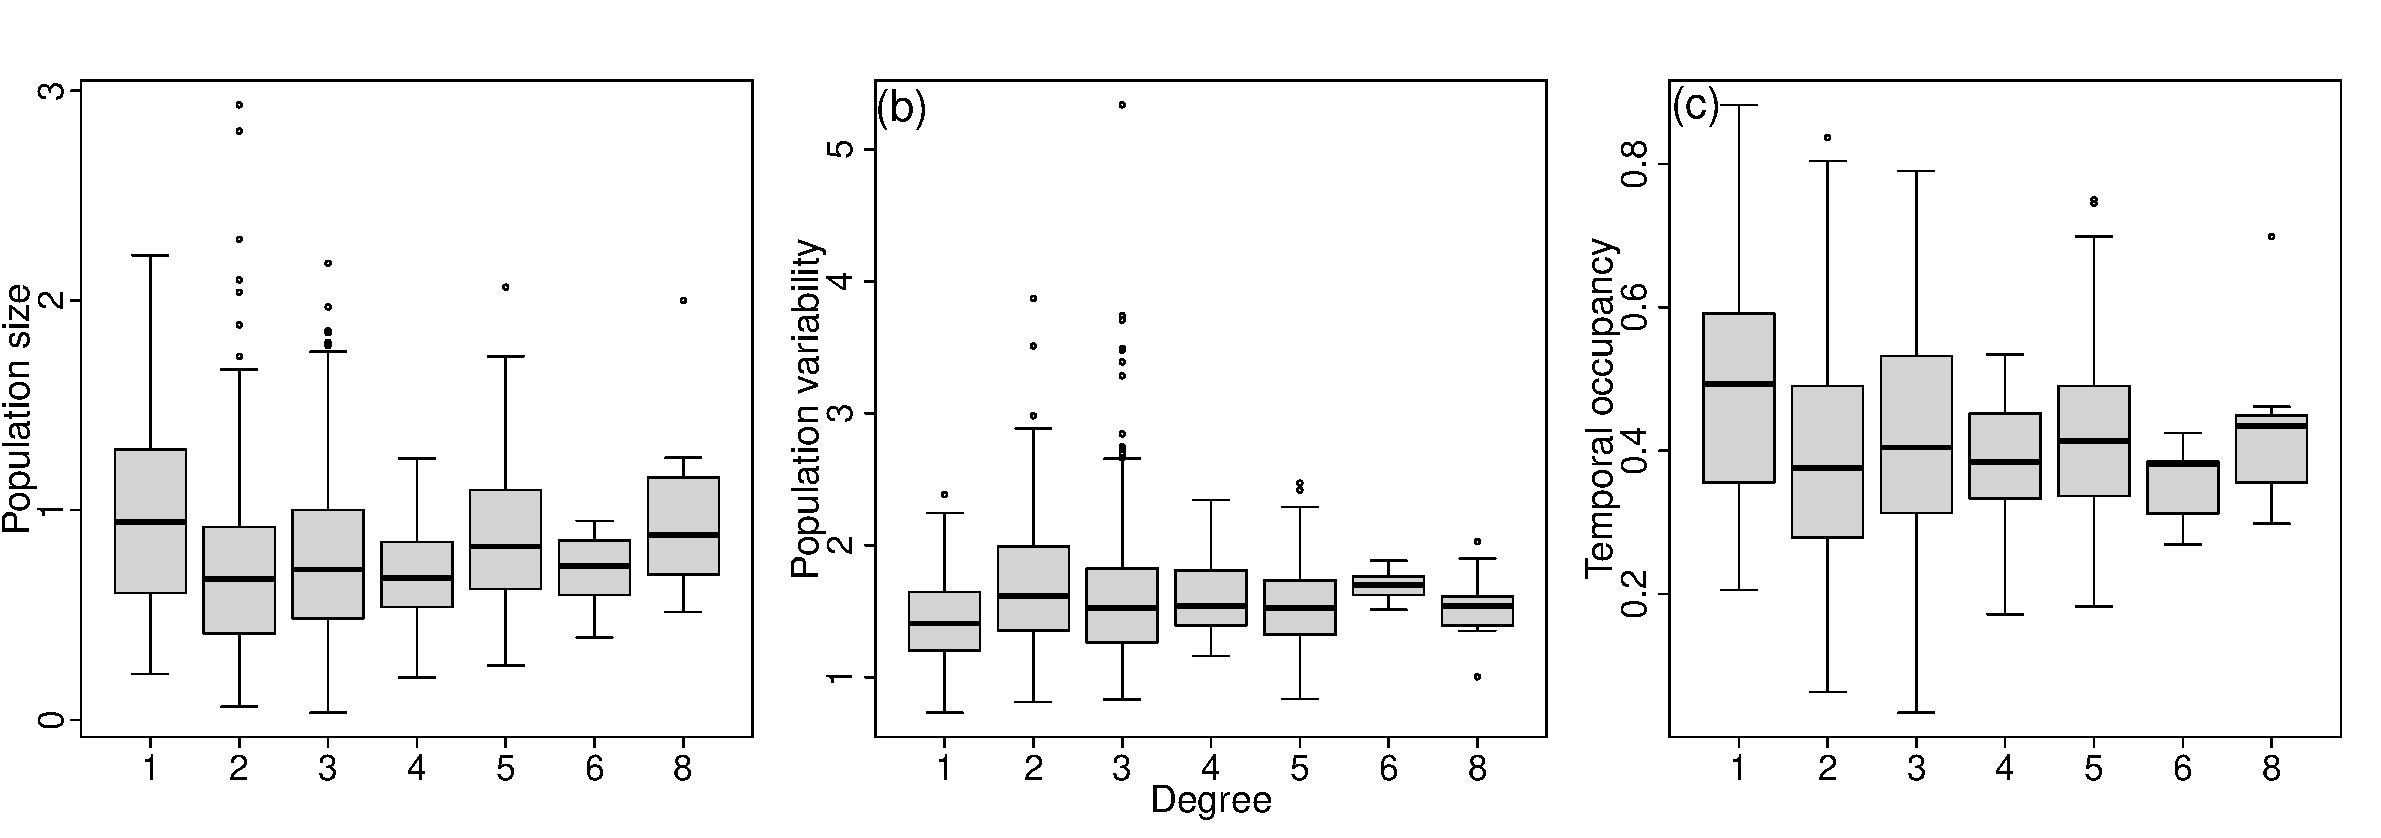
\includegraphics[width=1\textwidth]{FigSpat/pop_res}}
\caption[Effect of degree on local populations]{Degree did not affect local population size (a), local population variability (b), and the temporal occupancy of patches.} 
\label{fig:pop}
\end{figure}













